%\begin{comment}
\chapter{Data Validation Plots for $K_S^0$}

\begin{figure}[H]
\caption{The distribution of the training variables in KsFinder. The blue and purple solid lines are the total and true $K_S^0$ distributions from generic MC, respectively. The yellow and red dots are the data distribution before and after applying KsFinder cut. The uncertainties in data are taken as three times the Poisson standard deviation.}
\begin{subfigure}{0.5\linewidth}
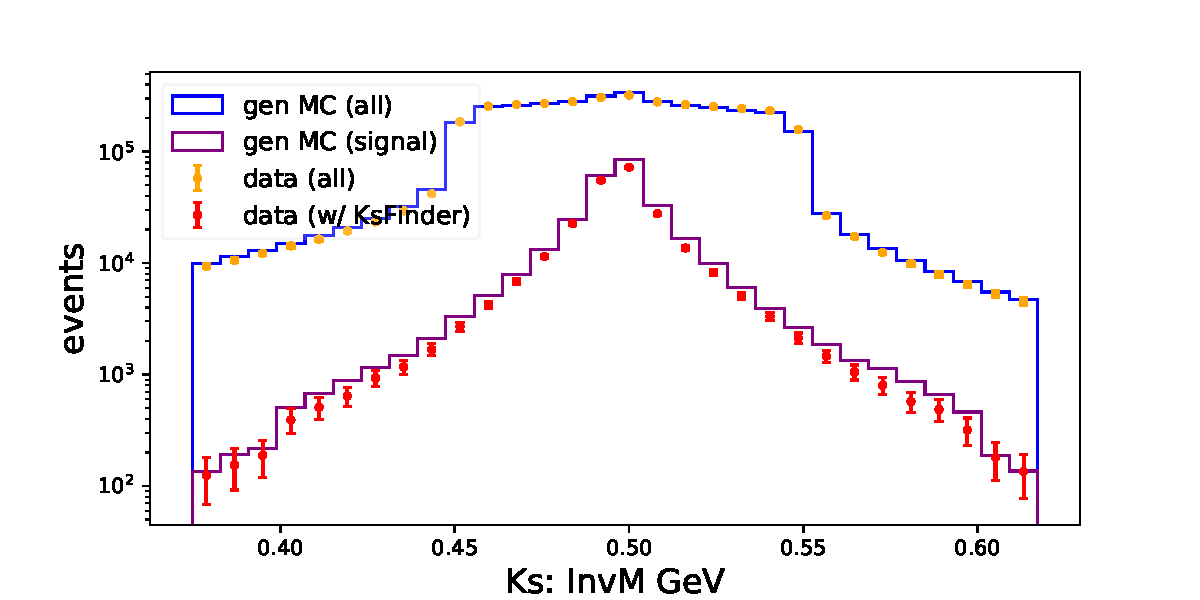
\includegraphics[page=1,width=1.1\linewidth]{dataVarsPlot_Ks.pdf}
\end{subfigure}
\begin{subfigure}{0.5\linewidth}
\includegraphics[page=2,width=1.1\linewidth]{dataVarsPlot_Ks.pdf}
\end{subfigure}
\end{figure}

%\begin{comment}
\begin{figure}[H]
\ContinuedFloat
\begin{subfigure}{0.5\linewidth}
	\includegraphics[page=3,width=1.1\linewidth]{dataVarsPlot_Ks.pdf}
\end{subfigure}
\begin{subfigure}{0.5\linewidth}
	\includegraphics[page=4,width=1.1\linewidth]{dataVarsPlot_Ks.pdf}
\end{subfigure}
\begin{subfigure}{0.5\linewidth}
	\includegraphics[page=5,width=1.1\linewidth]{dataVarsPlot_Ks.pdf}
\end{subfigure}
\begin{subfigure}{0.5\linewidth}
	\includegraphics[page=6,width=1.1\linewidth]{dataVarsPlot_Ks.pdf}
\end{subfigure}
\end{figure}

\begin{figure}[H]
\ContinuedFloat
\begin{subfigure}{0.5\linewidth}
	\includegraphics[page=7,width=1.1\linewidth]{dataVarsPlot_Ks.pdf}
\end{subfigure}
\begin{subfigure}{0.5\linewidth}
	\includegraphics[page=8,width=1.1\linewidth]{dataVarsPlot_Ks.pdf}
\end{subfigure}
\begin{subfigure}{0.5\linewidth}
	\includegraphics[page=9,width=1.1\linewidth]{dataVarsPlot_Ks.pdf}
\end{subfigure}
\begin{subfigure}{0.5\linewidth}
\includegraphics[page=10,width=1.1\linewidth]{dataVarsPlot_Ks.pdf}
\end{subfigure}
\end{figure}

\begin{figure}[H]
\ContinuedFloat
\begin{subfigure}{0.5\linewidth}
	\includegraphics[page=11,width=1.1\linewidth]{dataVarsPlot_Ks.pdf}
\end{subfigure}
\begin{subfigure}{0.5\linewidth}
	\includegraphics[page=12,width=1.1\linewidth]{dataVarsPlot_Ks.pdf}
\end{subfigure}
\begin{subfigure}{0.5\linewidth}
\includegraphics[page=13,width=1.1\linewidth]{dataVarsPlot_Ks.pdf}
\end{subfigure}
\begin{subfigure}{0.5\linewidth}
\includegraphics[page=14,width=1.1\linewidth]{dataVarsPlot_Ks.pdf}
\end{subfigure}
\end{figure}

%\begin{comment}
\begin{figure}[H]
	\ContinuedFloat
	\begin{subfigure}{0.5\linewidth}
		\includegraphics[page=15,width=1.1\linewidth]{dataVarsPlot_Ks.pdf}
	\end{subfigure}
	\begin{subfigure}{0.5\linewidth}
		\includegraphics[page=16,width=1.1\linewidth]{dataVarsPlot_Ks.pdf}
	\end{subfigure}
\begin{subfigure}{0.5\linewidth}
\includegraphics[page=17,width=1.1\linewidth]{dataVarsPlot_Ks.pdf}
\end{subfigure}
\begin{subfigure}{0.5\linewidth}
\includegraphics[page=18,width=1.1\linewidth]{dataVarsPlot_Ks.pdf}
\end{subfigure}

\end{figure}

\begin{figure}[H]
	\ContinuedFloat
\begin{subfigure}{0.5\linewidth}
	\includegraphics[page=19,width=1.1\linewidth]{dataVarsPlot_Ks.pdf}
\end{subfigure}
\begin{subfigure}{0.5\linewidth}
	\includegraphics[page=22,width=1.1\linewidth]{dataVarsPlot_Ks.pdf}
\end{subfigure}
\begin{subfigure}{0.5\linewidth}
	\includegraphics[page=23,width=1.1\linewidth]{dataVarsPlot_Ks.pdf}
\end{subfigure}
\begin{subfigure}{0.5\linewidth}
	\includegraphics[page=24,width=1.1\linewidth]{dataVarsPlot_Ks.pdf}
\end{subfigure}
\end{figure}

\begin{figure}[H]
	\ContinuedFloat
	\begin{subfigure}{0.5\linewidth}
		\includegraphics[page=25,width=1.1\linewidth]{dataVarsPlot_Ks.pdf}
	\end{subfigure}
\end{figure}
%\end{comment}

%\end{comment}

%\end{comment}
